\subsection{TS(M)与S(M)之间的关系}

M 到 TS(M) 中的典范单射以唯一方式延拓为 T(M) 到 TS(M) 中的一个代数同态（III，第 485 页，命题 1）。由 IV 第 43 页命题 2 (ii)，该同态就是对称化算子 s。由于代数 TS(M) 是交换的，因此存在（III，第 497 页）唯一的代数同态 \(\varphi_{M}\) （称为典范的），它从代数 S(M) 到代数 TS(M) 中，使得图表

\pandocbounded{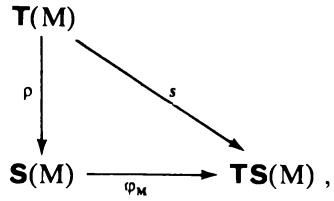
\includegraphics[keepaspectratio]{images/part001_42062a6f.jpg}}

，其中 \(\rho\) 表示 \(\mathbf{T}(\mathbf{M})\) 到 \(\mathbf{S}(\mathbf{M})\) 上的典范同态，图表交换。我们有 \(\varphi_{\mathbf{M}}(\mathbf{S}^{p}(\mathbf{M})) \subset \mathbf{T}\mathbf{S}^{p}(\mathbf{M})\) （对所有 \(p \in N\) ）。

另一方面，把 TS(M) 到 T(M) 的典范单射 i 与 T(M) 到 S(M) 的典范同态 \(\rho\) 复合，我们得到分次 A-模的一个同态 \(\psi_{M}\) ，称为典范的。图表

\pandocbounded{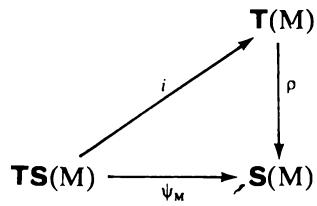
\includegraphics[keepaspectratio]{images/part001_38781a0a.jpg}}

是交换的。

如果 \(u: \mathbf{M} \to \mathbf{N}\) 是A-模的同态，则图表

\begin{enumerate}
\def\labelenumi{(\arabic{enumi})}
\setcounter{enumi}{12}
\tightlist
\item
\end{enumerate}

\pandocbounded{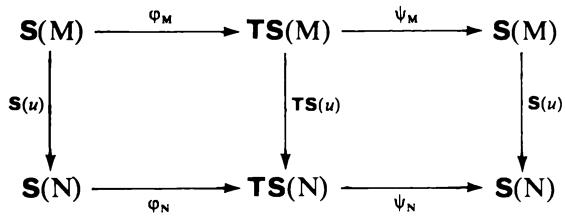
\includegraphics[keepaspectratio]{images/part001_026b2058.jpg}}

是交换的，这很容易验证。

若M是模 \(M_{\lambda}\) 的直和，则图表

\begin{enumerate}
\def\labelenumi{(\arabic{enumi})}
\setcounter{enumi}{13}
\tightlist
\item
\end{enumerate}

\pandocbounded{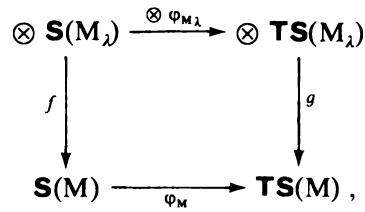
\includegraphics[keepaspectratio]{images/part001_9b5b14d2.jpg}}

，其中 \(f\) 和 \(g\) 是典范同态，是交换的。因为 \(g \circ \bigotimes_{\lambda} \varphi_{M_{\lambda}}\) 与 \(\varphi_{M} \circ f\) 都是代数同态，且它们在 \(M_{\lambda}\) 上（对每个 \(\lambda\) ）取值一致。

命题 11. --- 若 M 是自由的，则 \(\varphi_{\mathbf{M}}\) 是分次双代数的一个态射。

利用图表（13）和（14）的交换性，我们得到交换图表

\[
\begin{array}{l} \mathbf {S} (\mathrm{M}) \xrightarrow {\mathbf {S} (\Delta)} \mathbf {S} (\mathrm{M} \oplus \mathrm{M}) \xrightarrow {h} \mathbf {S} (\mathrm{M}) \otimes \mathbf {S} (\mathrm{M}) \\ \varphi_ {\mathrm{M}} \Bigg | _ {\downarrow} \quad \Bigg | _ {\varphi_ {\mathrm{M}} \oplus \mathrm{M}} \quad \Bigg | _ {\varphi_ {\mathrm{M}} \otimes \varphi_ {\mathrm{M}}} \\ \mathbf {T S} (\mathrm{M}) \xrightarrow [ \mathsf {T S} (\Delta) ]{} \mathbf {T S} (\mathrm{M} \oplus \mathrm{M}) \xrightarrow [ k ]{} \mathbf {T S} (\mathrm{M}) \cdot \otimes \mathbf {T S} (\mathrm{M}), \end{array}
\]

，其中 \(\Delta\) 是对角同态，而 h、k 是典范同态。命题由此得证。

命题 12. --- (i) 若 \(u \in \mathbf{S}^n(\mathbf{M})\) ，则 \(\psi_{\mathbf{M}}(\varphi_{\mathbf{M}}(u)) = n!u\) 。

\begin{enumerate}
\def\labelenumi{(\roman{enumi})}
\setcounter{enumi}{1}
\tightlist
\item
  若 \(v \in \mathbf{T}\mathbf{S}^n(\mathbf{M})\) ，则 \(\varphi_{\mathbf{M}}(\psi_{\mathbf{M}}(v)) = n!v\) 。
\end{enumerate}

设 \(x_{1}, \ldots, x_{n} \in M\) ，并令 u 为乘积 \(x_{1} \ldots x_{n}\) （在 \(\mathbf{S}(\mathbf{M})\) 中计算的）。则 \(\varphi_{\mathbf{M}}(u)\) 是乘积 \(x_{1} \ldots x_{n}\) （在 \(\mathbf{T}\mathbf{S}(\mathbf{M})\) 中计算的），即

\[
\sum_ {\sigma \in \mathfrak {S} _ {n}} x _ {\sigma (1)} \otimes \dots \otimes x _ {\sigma (n)}.
\]

因此 \(\psi_{\mathbf{M}}(\varphi_{\mathbf{M}}(u))\) 等于 \(\sum_{\sigma \in \mathfrak{S}_n}x_{\sigma (1)}\ldots x_{\sigma (n)}\) （在 \(\mathbf{S}(\mathbf{M})\) 中计算的），即

\[
n! x _ {1} \dots x _ {n} = n! u.
\]

设 \(v = \sum_{i=1}^{p} x_1^i \otimes x_2^i \otimes \ldots \otimes x_n^i\) 为 \(\mathbf{TS}^n(\mathbf{M})\) 的一个元素，其中 \(x_j^i\) 属于

\(\mathbf{M}\) ；则 \(\psi_{\mathbf{M}}(v)\) 等于 \(\sum_{i=1}^{p} x_1^i x_2^i \ldots x_n^i\) （在 \(\mathbf{S}(\mathbf{M})\) 中计算的），从而

\[
\varphi_ {\mathrm{M}} \big (\psi_ {\mathrm{M}} (v) \big) = \sum_ {i = 1} ^ {p} \mathbf {s} \big (x _ {1} ^ {i} \otimes x _ {2} ^ {i} \otimes \dots \otimes x _ {n} ^ {i} \big) = s (v) = n! v.
\]

推论 1. --- 若 A 是 Q-代数，则 S(M) 到 TS(M) 的典范同态是代数同构。若进一步 M 是自由的，则它是分次双代数的同构。

推论 2. --- 若 A 是一个 Q-代数，则模 \(\mathbf{TS}^n (\mathbf{M})\) 由 \(n\) 次幂（\(\mathbf{M}\) 的元素在 \(\mathbf{TS}(\mathbf{M})\) 中的）生成。

这由推论 1 及 \(\mathbf{S}(\mathbf{M})\) 的相应性质（III，第 498 页）得出。

